\documentclass[tikz,border=6pt]{standalone}
% shared TikZ style for the diagrams (colours match the plots)
\usepackage[T1]{fontenc}
\usepackage{lmodern}
\usepackage{amsmath,amssymb}
\usepackage{tikz}
\usetikzlibrary{arrows.meta,positioning,fit,backgrounds,calc,shapes.misc,decorations.pathreplacing}
\definecolor{cBlue}{HTML}{2A78D6}
\definecolor{cOrange}{HTML}{EB6834}
\definecolor{cAqua}{HTML}{1BAF7A}
\definecolor{cViolet}{HTML}{6250D6}
\definecolor{cGreen}{HTML}{008300}
\definecolor{cGray}{HTML}{8F8D86}
\definecolor{cInk}{HTML}{0B0B0B}
\definecolor{cInk2}{HTML}{52514E}
\tikzset{
  box/.style={draw=#1!70!black, fill=#1!10, rounded corners=3pt, align=center, inner sep=4pt, font=\small, line width=0.6pt},
  box/.default=cGray,
  arr/.style={-{Stealth[length=2.4mm]}, line width=0.8pt, cInk2},
  lbl/.style={font=\scriptsize, text=cInk2, align=center},
}

% 8 x 16 weight matrix, V=4 rows x M=8 columns per block -> 2 x 2 blocks.
% \blockgrid{row-block}{col-block}{kept columns}{mode: 1 = vector step only, 2 = + 2:4 inside kept columns}
\newcommand{\blockgrid}[4]{%
  \foreach \r in {0,...,3}{\foreach \c in {0,...,7}{\fill[gray!12] (#2*2.56+\c*0.32,-#1*1.28-\r*0.32) rectangle ++(0.3,-0.3);}}
  \foreach \c [count=\i from 0] in {#3}{\foreach \r in {0,...,3}{
    \pgfmathsetmacro{\keep}{int(mod(\i+\r+#1+#2,4)<2)}
    \ifnum#4=1 \fill[cOrange!55] (#2*2.56+\c*0.32,-#1*1.28-\r*0.32) rectangle ++(0.3,-0.3);
    \else\ifnum\keep=1 \fill[cAqua] (#2*2.56+\c*0.32,-#1*1.28-\r*0.32) rectangle ++(0.3,-0.3);
    \else \fill[cOrange!25] (#2*2.56+\c*0.32,-#1*1.28-\r*0.32) rectangle ++(0.3,-0.3); \fi\fi}}}
\newcommand{\allblocks}[1]{\blockgrid{0}{0}{1,2,5,7}{#1}\blockgrid{0}{1}{0,3,4,6}{#1}%
  \blockgrid{1}{0}{0,2,3,6}{#1}\blockgrid{1}{1}{1,4,5,7}{#1}}
\newcommand{\frameblocks}{%
  \draw[cInk, line width=0.9pt] (-0.02,0.02) rectangle (5.12,-2.58);
  \draw[cInk, line width=0.9pt] (2.55,0.02)--(2.55,-2.58); \draw[cInk, line width=0.9pt] (-0.02,-1.27)--(5.12,-1.27);}
\begin{document}
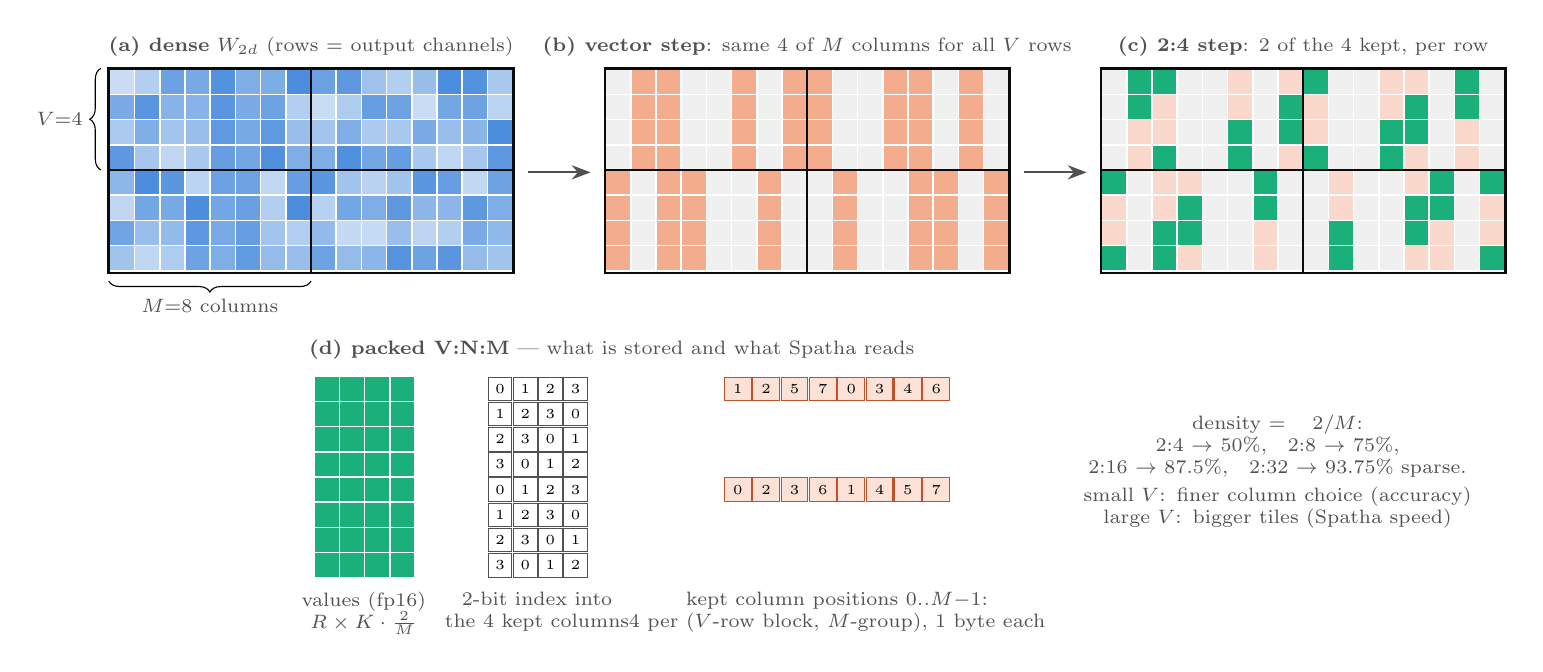
\begin{tikzpicture}[x=1cm,y=1cm]
% ---------- (a) dense
\begin{scope}
\foreach \r in {0,...,7}{\foreach \c in {0,...,15}{
  \pgfmathsetmacro{\s}{int(mod(37*\r+11*\c*\c+5*\r*\c,60)+25)}
  \fill[cBlue!\s] (\c*0.32,-\r*0.32) rectangle ++(0.3,-0.3);}}
\frameblocks
\node[lbl, above] at (2.55,0.05) {\textbf{(a) dense} $W_{2d}$ (rows = output channels)};
\draw[decorate,decoration={brace,amplitude=4pt}] (-0.12,-1.27)--(-0.12,0.02) node[midway,left=3pt,lbl]{$V{=}4$};
\draw[decorate,decoration={brace,amplitude=4pt,mirror}] (-0.02,-2.68)--(2.55,-2.68) node[midway,below=3pt,lbl]{$M{=}8$ columns};
\end{scope}
% ---------- (b) vector step
\begin{scope}[xshift=6.3cm]
\allblocks{1}\frameblocks
\node[lbl, above] at (2.55,0.05) {\textbf{(b) vector step}: same 4 of $M$ columns for all $V$ rows};
\end{scope}
% ---------- (c) 2:4 step
\begin{scope}[xshift=12.6cm]
\allblocks{2}\frameblocks
\node[lbl, above] at (2.55,0.05) {\textbf{(c) 2:4 step}: 2 of the 4 kept, per row};
\end{scope}
\draw[arr] (5.3,-1.3)--(6.1,-1.3); \draw[arr] (11.6,-1.3)--(12.4,-1.3);
% ---------- (d) packed storage
\begin{scope}[yshift=-3.9cm, xshift=2.6cm]
\node[lbl, anchor=west] at (-0.2,0.35) {\textbf{(d) packed V:N:M} --- what is stored and what Spatha reads};
\foreach \r in {0,...,7}{\foreach \c in {0,...,3}{\fill[cAqua] (\c*0.32,-\r*0.32) rectangle ++(0.3,-0.3);}}
\node[lbl, below] at (0.62,-2.6) {values (fp16)\\$R\times K\cdot\tfrac{2}{M}$};
\foreach \r in {0,...,7}{\foreach \c in {0,...,3}{\draw[cInk2, fill=white] (2.2+\c*0.32,-\r*0.32) rectangle ++(0.3,-0.3);
  \pgfmathsetmacro{\v}{int(mod(\c+\r,4))}\node[font=\tiny] at (2.35+\c*0.32,-\r*0.32-0.15) {\v};}}
\node[lbl, below] at (2.82,-2.6) {2-bit index into\\the 4 kept columns};
\foreach \rb/\ids in {0/{1,2,5,7,0,3,4,6}, 1/{0,2,3,6,1,4,5,7}}{
  \foreach \v [count=\c from 0] in \ids {\draw[cOrange!80!black, fill=cOrange!20] (5.2+\c*0.36,-\rb*1.28) rectangle ++(0.34,-0.3);
    \node[font=\tiny] at (5.37+\c*0.36,-\rb*1.28-0.15) {\v};}}
\node[lbl, below] at (6.63,-2.6) {kept column positions $0..M{-}1$:\\4 per ($V$-row block, $M$-group), 1 byte each};
\node[lbl, anchor=west, text width=58mm] at (9.2,-1.2) {density $=2/M$:\\2:4 $\to$ 50\%, \; 2:8 $\to$ 75\%,\\2:16 $\to$ 87.5\%, \; 2:32 $\to$ 93.75\% sparse.\\[2pt] small $V$: finer column choice (accuracy)\\large $V$: bigger tiles (Spatha speed)};
\end{scope}
\end{tikzpicture}
\end{document}
